\documentclass[10pt,aspectratio=169]{beamer}
% compile: pdflatex presentation_pt.tex  (run twice from inside docs/)
% or push to GitHub -- .github/workflows/ compila automaticamente.

\usepackage[utf8]{inputenc}
\usepackage[T1]{fontenc}
\usepackage{lmodern}
\usepackage[portuguese]{babel}
\usepackage{amsmath}
\usepackage{amssymb}
\usepackage{booktabs}
\usepackage{array}
\usepackage{graphicx}
\usepackage{grffile}
\usepackage{xcolor}
\usepackage{tikz}
\usetikzlibrary{arrows.meta,shapes,positioning}

\usetheme{Berlin}
\usecolortheme{seahorse}
\setbeamertemplate{footline}[frame number]
\setbeamertemplate{navigation symbols}{}

\newcommand{\bk}{\hfill\hyperlink{toc}{\beamerreturnbutton{Agenda}}}
\newcommand{\miplink}{\hyperlink{mip1}{\beamergotobutton{Modelo MIP completo (ap\^endice)}}}

\title{\large Planeamento de Cirurgias Electivas}
\subtitle{Programa\c{c}\~ao por restri\c{c}\~oes baseada em intervalos (CP-SAT)
  para planeamento semanal de blocos operatórios}
\author{Hector Bonilla}
\date{}

\begin{document}

\begin{frame}\titlepage\end{frame}

\begin{frame}{Agenda}
  \hypertarget{toc}{}
  \tableofcontents
  \vspace{0.5em}
  \footnotesize Fluxo principal: modelo CP-SAT completo -- variáveis,
  parâmetros e restrições em detalhe. O modelo MIP de comparação
  está no apêndice -- é evidência para a escolha CP-SAT, não um
  segundo modelo a apresentar.
\end{frame}

% ============================================================
\section{Problema e Motivação}

\begin{frame}{O problema}
  \textbf{Um hospital, uma semana. Uma lista de espera cirúrgica sempre
  maior do que a capacidade semanal dos blocos operatórios.}
  \begin{itemize}\small
    \item Para cada caso em espera: qual bloco, qual dia, que hora,
      qual cirurgião -- ou adiar para a semana seguinte.
    \item \textbf{Viabilidade}: blocos, cirurgiões, equipamento partilhado
      e camas de recuperação são todos finitos e partilhados.
    \item \textbf{Equidade clínica}: a urgência clínica, e não a ordem
      de chegada, deve determinar prioridade -- um doente genuinamente
      urgente não pode ficar atrás de um caso rotineiro.
    \item \textbf{Âmbito (Cardoen et al., 2010):} este é o problema de
      \emph{planeamento antecipado} -- atribuição de casos a dias/blocos
      com antecedência -- distinto da sequenciação intra-dia e da gestão
      de perturbações em tempo real.
  \end{itemize}
\end{frame}

\begin{frame}{Porquê é importante}
  \begin{itemize}\small
    \item \textbf{O tempo de bloco operatório é caro e perecível.}
      $\sim\$30$--$40$/minuto uma vez amortizados pessoal, equipamento
      e overhead (Macario, 2010). Um minuto de bloco inactivo hoje
      não pode ser guardado para amanhã.
    \item \textbf{A lista de espera é o indicador auditado.}
      Em sistemas como o SIGIC português, o RTT do NHS britânico e os
      benchmarks provinciais canadianos, a taxa de incumprimento dos prazos
      é o número que é publicado e pelo qual o planeador é avaliado.
    \item \textbf{Procura electiva e urgente partilham os mesmos blocos}
      (Van Riet \& Demeulemeester, 2015) -- a alocação de capacidade é
      uma decisão estratégica, não um subproduto do agendamento.
    \item \textbf{Evidência na literatura:} Cardoen, Demeulemeester
      \& Beli\"en (2010) revêem mais de 200 artigos; o planeamento
      antecipado com restrições de prioridade/prazo é um sub-problema
      bem definido, que este projecto ocupa na sua totalidade.
  \end{itemize}
\end{frame}

\begin{frame}{O caso português: o sistema SIGIC}
  \textbf{SIGIC} -- \emph{Sistema Integrado de Gestão de Inscritos para
  Cirurgia} -- é o sistema nacional português de gestão da lista de espera
  cirúrgica, estabelecido pela \textbf{Portaria n.\textsuperscript{o}
  45/2008} (Diário da República).

  \vspace{0.5em}
  Cada caso electivo é classificado numa de \textbf{quatro prioridades
  clínicas}, com um \textbf{tempo máximo de espera} associado:

  \vspace{0.4em}
  \begin{center}\small
  \begin{tabular}{clc}
    \toprule
    Prioridade & Significado clínico & Espera máxima (dias) \\
    \midrule
    1 & Electivo de rotina & 270 \\
    2 & Urgência elevada & 60 \\
    3 & Urgente & 15 \\
    4 & Emergente/adicional -- deve operar esta semana & 3 \\
    \bottomrule
  \end{tabular}
  \end{center}
  \vspace{0.4em}
  \footnotesize Estes quatro números \emph{não} são valores ilustrativos
  inventados para a demo -- são os parâmetros $\text{wl}^{max}_p$ do modelo,
  retirados directamente de uma política legislada e auditada.
\end{frame}

\begin{frame}{O caso português: a auditoria CHLN de 2016}
  Marques \& Captivo (2015) auditaram a lista de espera do Centro Hospitalar
  Lisboa Norte (CHLN) face às metas SIGIC. Principais conclusões:

  \begin{itemize}\small
    \item $\sim$\textbf{7\,400} doentes na lista no momento da auditoria.
    \item \textbf{16\%} já tinha \emph{ultrapassado} o prazo máximo da
      respectiva prioridade.
    \item Atraso médio entre os casos em incumprimento: \textbf{147 dias}
      a nível hospitalar.
    \item Neurocirurgia: atraso médio de $\sim$\textbf{261 dias} -- muito
      acima da média hospitalar.
  \end{itemize}
  \pause
  \begin{block}{Porque é que isto molda o objectivo deste modelo}
    Um planeador que optimize apenas o volume pode apresentar uma excelente
    utilização e reproduzir silenciosamente o modo de falha desta auditoria
    -- agendando casos de rotina e adiando os casos em incumprimento
    indefinidamente. O termo de penalização $w_c$ no objectivo existe
    precisamente para tornar estes custos \emph{explícitos, ponderados
    e dominantes}.
  \end{block}
\end{frame}

% ============================================================
\section{Pressupostos e Âmbito}

\begin{frame}{O que o modelo cobre -- e o que não cobre}
  \begin{columns}
    \begin{column}{0.5\textwidth}
      \textbf{Modelado:}
      \begin{itemize}\small
        \item Atribuição caso$\to$bloco$\to$hora$\to$cirurgião
        \item Escalas de serviço dos blocos (block schedule)
        \item Disponibilidade e limites horários dos cirurgiões
        \item Uma unidade de imagiologia partilhada (intensificador C)
        \item Camas de recuperação/UCI (internamento multi-dia)
        \item Bloqueio de prioridade 4 (dia 1)
        \item Regra de bloco pediátrico
      \end{itemize}
    \end{column}
    \begin{column}{0.5\textwidth}
      \textbf{Excluído deliberadamente:}
      \begin{itemize}\small
        \item Duções estocásticas
        \item Perturbações intra-dia
        \item Escalonamento de enfermeiros/anestesistas
        \item Limpeza dependente da sequência
        \item Horizonte multi-semana
        \item Dimensionamento de reserva para urgências
        \item Preferências dos doentes por dia
      \end{itemize}
    \end{column}
  \end{columns}
\end{frame}

\begin{frame}{Pressupostos chave -- detalhe e justificação}
  \small
  \begin{enumerate}
    \item \textbf{Durações determinísticas.} Uma duração por caso (ex.:
      mediana histórica do procedimento). As durações reais são estocásticas
      e tendem a ser subestimadas; o caso determinístico é a aproximação
      tratável padrão (Denton et al., 2010). A extensão estocástica
      requer programação estocástica de dois estágios.
    \item \textbf{Limpeza por escalão de duração} (15/25/40 min):
      proxy para o intervalo real de 15--60 min; captura a componente
      correlacionada com a duração, não a dependente da sequência.
    \item \textbf{Cirurgiões como recurso de pessoal limitante.}
      Enfermeiros/anestesistas assumidos com o bloco -- válido quando
      a agenda do cirurgião é o verdadeiro bottleneck.
    \item \textbf{Uma ocorrência por doente por semana.} Padrão conservador;
      combinar procedimentos no mesmo dia é julgamento clínico específico
      do serviço.
    \item \textbf{Capacidade de camas constante na semana}, com penalização
      de transbordo explícita -- sem aproximação silenciosa.
    \item \textbf{Bloco pediátrico} como exemplo de regra institucional
      ad hoc: apenas um predicado de elegibilidade, sem novas variáveis.
    \item \textbf{Uma semana, um hospital, sem perturbações intra-dia} --
      planeamento antecipado apenas.
  \end{enumerate}
\end{frame}

% ============================================================
\section{Dados e Instâncias}

\begin{frame}{Modelo de dados}
  A camada de dados (\texttt{src/model/types.py}) é independente do solver
  -- dataclasses Python simples, sem importações do solver.

  \begin{itemize}\small
    \item \textbf{\texttt{SurgicalCase}}: id do doente, serviço, cirurgião,
      prioridade $p_c$, dias em espera $\text{wl}_c$, tempo operatório
      $t_c^{op}$, limpeza $t_c^{clean}$, equipamento opcional, cama opcional.
    \item \textbf{\texttt{Surgeon}}: limite diário $k_{hd}$, limite semanal
      $k_h$, disponibilidade por dia.
    \item \textbf{\texttt{OperatingRoom}}: capacidade por dia $k_{dr}$,
      escala de serviço, flag de ambulatório.
    \item \textbf{\texttt{PlanningInstance}}: agrega tudo acima mais os
      parâmetros de política ($\text{wl}^{max}_p$, $\mu_p$, $\alpha$,
      capacidades de equipamento/cama, regra pediátrica).
  \end{itemize}
  \vspace{0.4em}
  Cada solver lê \texttt{PlanningInstance} e devolve
  \texttt{SolverResult} -- o padrão adaptador que torna os backends
  intercambiáveis.
\end{frame}

\begin{frame}{demo\_instance() -- 20 casos, 5 blocos, 6 cirurgiões}
  \small 3 serviços: ORL (otorrinolaringologia), ORTHO (ortopedia),
  VASC (cirurgia vascular).

  \begin{center}
  \begin{tabular}{lccc}
    \toprule
    Serviço & Blocos & Capacidade (min/dia) & Cirurgiões \\
    \midrule
    ORL   & 2 & 360 ($\approx$ 6 h) & 2 \\
    ORTHO & 1 & 450 ($\approx$ 7.5 h) & 1 \\
    VASC  & 2 & 660 ($\approx$ 11 h) & 3 \\
    \bottomrule
  \end{tabular}
  \end{center}
  \vspace{0.3em}
  Características especiais activadas (uma por família de restrições):
  \begin{itemize}\footnotesize
    \item 3 casos prioridade-4 (C05 ORL, C13 ORTHO, C19 VASC) -- bloqueados à 2ª feira
    \item Intensificador C partilhado, capacidade 1/dia (VASC endovascular: C14, C15, C17, C19)
    \item 2 camas de UCI/dia; C14 e C16 necessitam de 1 dia de internamento
    \item Bloco pediátrico: 6ª feira no serviço ORL restrito a idade $\le 8$
    \item 3 casos em incumprimento (C03, C11, C16) -- já ultrapassaram o prazo SIGIC
  \end{itemize}
  \footnotesize Dimensionada para ser lida de vista e para exercitar
  \emph{todas} as famílias de restrições numa execução.
\end{frame}

\begin{frame}{medium\_instance() -- 200 casos, 12 blocos, 17 cirurgiões}
  \small 5 serviços; estrutura inspirada na família de benchmarks
  multi-serviço de Cardoen et al. (2010).

  \begin{center}
  \begin{tabular}{lcccc}
    \toprule
    Serviço & Blocos & Cap. (min/d) & Cirurgiões & Equipamento \\
    \midrule
    ORL   & 2 & 360 & 3 & -- \\
    ORTHO & 3 & 480 & 4 & -- \\
    VASC  & 2 & 660 & 3 & Intensificador C \\
    GIN   & 2 & 300 & 3 & -- \\
    NEURO & 3 & 540 & 4 & Intensificador C \\
    \bottomrule
  \end{tabular}
  \end{center}
  \begin{itemize}\footnotesize
    \item Mix de prioridades: 58\% P1 / 26\% P2 / 13\% P3 / 3\% P4
    \item $\sim$40\% dos cirurgiões têm uma folga/semana (nunca 2ª feira)
    \item 12\% dos casos VASC/NEURO necessitam de cama UCI (1--2 dias)
    \item Limites dos cirurgiões: 300 min/dia, 1300 min/semana
  \end{itemize}
  \footnotesize Usada para demonstrar escalabilidade e medir o desfasamento
  CP-vs-MIP (secção de resultados).
\end{frame}

\begin{frame}{Disponibilidade de dados reais}
  As instâncias sintéticas acima são estruturalmente calibradas. Existem
  dois conjuntos de dados hospitalares reais com licença aberta que se
  mapeiam directamente para \texttt{PlanningInstance} sem qualquer
  alteração à formulação:

  \begin{itemize}\small
    \item Akbarzadeh \& Maenhout (2023a).
      \emph{Real life data for OR scheduling}
      -- registo de blocos do Hospital Universitário de Ghent, Maio 2017.
      Mendeley Data V2.
      \texttt{doi:10.17632/n2v49z2vnp.2}
    \item Akbarzadeh \& Maenhout (2023b).
      \emph{RealLife OR scheduling dataset, 2021-Jan-May}
      -- 20 instâncias semanais, 8 configurações.
      Mendeley Data V1.
      \texttt{doi:10.17632/c8d342266x.1}
  \end{itemize}
  \footnotesize Ambos são CC~BY~4.0 e contêm o mesmo esquema de escala
  mestre + lista de espera por caso usado por \texttt{PlanningInstance}.
  Um deployment real começaria aqui.
\end{frame}

% ============================================================
\section{Modelo CP-SAT}

\begin{frame}{Conjuntos e índices}
  \begin{center}\small
  \begin{tabular}{cl}
    \toprule
    Símbolo & Significado \\
    \midrule
    $c \in C$ & Casos cirúrgicos (um por par doente-procedimento) \\
    $d \in D$ & Dias de planeamento, $D=\{1,\dots,5\}$ (2\textordfeminine--6\textordfeminine feira) \\
    $r \in R$ & Blocos operatórios \\
    $h \in H$ & Cirurgiões \\
    $e \in E$ & Tipos de equipamento partilhado \\
    $D_c \subseteq D$ & Dias elegíveis para o caso $c$; $\{1\}$ se prioridade-4 \\
    \bottomrule
  \end{tabular}
  \end{center}
  \vspace{0.5em}
  \footnotesize Os candidatos $(c,d,r)$ são pré-filtrados por
  elegibilidade (C4--C6) \emph{antes} de qualquer variável ser criada
  -- esta é a principal redução do número de variáveis, não uma
  restrição adicional.
\end{frame}

\begin{frame}{Parâmetros (I): tempo, capacidade, prioridade}
  \small
  \begin{center}
  \begin{tabular}{cll}
    \toprule
    Símbolo & Significado & Valor padrão / origem \\
    \midrule
    $t_c^{op}$ & Duração operatória (min) & Mediana histórica \\
    $t_c^{clean}$ & Limpeza (min) & 15/25/40 por escalão de duração \\
    $t_c^{tot}=t_c^{op}+t_c^{clean}$ & Ocupação total do bloco & --- \\
    $k_{dr}$ & Minutos de abertura do bloco $r$ no dia $d$ & Escala hospitalar \\
    $k_{hd}$ & Limite operatório diário do cirurgião (min) & 240 (demo) / 300 (médio) \\
    $k_h$ & Limite operatório semanal do cirurgião (min) & 960 (demo) / 1300 (médio) \\
    $p_c\in\{1,2,3,4\}$ & Prioridade clínica & Triagem SIGIC \\
    $\text{wl}_c$ & Dias em espera (data de planeamento) & Dados hospitalares \\
    $\text{wl}^{max}_p$ & Espera máxima para prioridade $p$ & 270/60/15/3 (SIGIC) \\
    $dd_c=\text{wl}^{max}_{p_c}-\text{wl}_c$ & Folga ao prazo ($<0$ = incumprimento) & Calculado \\
    \bottomrule
  \end{tabular}
  \end{center}
\end{frame}

\begin{frame}{Parâmetros (II): objectivo e recursos partilhados}
  \small
  \begin{center}
  \begin{tabular}{cll}
    \toprule
    Símbolo & Significado & Valor padrão / origem \\
    \midrule
    $\mu_p$ & Multiplicador de prioridade & $\text{wl}^{max}_1/\text{wl}^{max}_p$ (derivado) \\
    $w_c$ & Penalização por não agendamento & $\mu_{p_c}\cdot\text{PenaltyCurve}(dd_c)+1.2\max dd$ \\
    $\alpha>1$ & Amplificador de urgência para casos em atraso & 2.0 (controlo de ordem) \\
    $u_{ce}\in\{0,1\}$ & 1 se o caso $c$ necessita do equipamento $e$ & Dados da instância \\
    $\kappa_{ed}$ & Capacidade simultânea do equip. $e$ no dia $d$ & 1 (demo), 2 (médio) \\
    $\rho(c)$ & Pool de camas necessária (``none'' se não aplicável) & Dados da instância \\
    $\text{los}_c$ & Dias de internamento nessa pool & Dados da instância \\
    $\beta_\rho$ & Número de camas na pool $\rho$ (constante/semana) & 2 (demo), 6 (médio) \\
    $\pi^{ovf}$ & Penalização/dia por estadia além do horizonte & 50 (configurável) \\
    \bottomrule
  \end{tabular}
  \end{center}
  \footnotesize $\mu_p$: prioridade autorizada a apenas $1/12$ da espera de P1
  é 12$\times$ mais sensível ao tempo de espera: $\mu_2=270/60=4.5$,
  $\mu_3=270/15=18$, $\mu_4=270/3=90$.
\end{frame}

\begin{frame}{Variáveis de decisão -- presença e agendamento}
  Para cada $(c,d,r)$ que passa na elegibilidade:
  \[\small
    \text{pr}_{cdr}\in\{0,1\}, \qquad
    \text{start}_{cdr},\,\text{end}_{cdr}\in[0,\,k_{dr}]
  \]
  Para cada caso que não é prioridade-4:
  \[\small
    u_c\in\{0,1\}, \qquad
    \sum_{d\in D_c,\,r}\text{pr}_{cdr} + u_c = 1
  \]
  \begin{itemize}\small
    \item $\text{pr}_{cdr}=1$: o caso $c$ é agendado no dia $d$ no bloco $r$.
    \item $u_c=1$: o caso $c$ \emph{não} é agendado esta semana e incorre
      na penalização $w_c$.
    \item Os casos de prioridade-4 não têm $u_c$: são forçados a ser
      agendados (restrição C2).
    \item Apenas os trios $(c,d,r)$ que passam C4--C6 têm variável --
      principal redução do número de variáveis.
  \end{itemize}
\end{frame}

\begin{frame}{Variáveis de decisão -- dois intervalos por candidato}
  \[\small
    \text{iv}_{cdr}=\texttt{NewOptionalIntervalVar}(\text{start}_{cdr},\;t_c^{tot},\;\text{end}_{cdr},\;\text{pr}_{cdr})
    \;\text{(BLOCO)}
  \]
  \[\small
    \text{sgiv}_{cdr}=\texttt{NewOptionalIntervalVar}(\text{start}_{cdr},\;t_c^{op},\;\text{sgend}_{cdr},\;\text{pr}_{cdr})
    \;\text{(CIRURGIÃO)}
  \]
  Ambos partilham \texttt{start}; ambos estão \emph{presentes} (restringem
  o recurso) exactamente quando $\text{pr}_{cdr}=1$.
  \pause
  \begin{block}{Porquê dois intervalos e não um?}
    \small O cirurgião H opera o Caso X: $t_c^{op}=70$, $t_c^{clean}=20$,
    início em $t=0$. O \emph{bloco} fica ocupado até $t=90$. O
    \emph{cirurgião} fica livre em $t=70$ e pode entrar no Bloco 2 para o
    Caso Y enquanto os enfermeiros terminam a limpeza do Bloco 1.
    Usar um único intervalo de tamanho $t_c^{tot}$ para C8 proibiria
    incorrectamente esta situação. Separar C7 (bloco, $t_c^{tot}$) de
    C8 (cirurgião, $t_c^{op}$) com o mesmo \texttt{start} resolve isto sem
    restrições de ligação explícitas.
  \end{block}
\end{frame}

\begin{frame}{Variáveis CP-SAT -- referência formal completa}
  \tiny
  \begin{center}
  \begin{tabular}{p{3.0cm}p{3.0cm}p{6.0cm}}
    \toprule
    \textbf{Variável} & \textbf{Domínio} & \textbf{Significado} \\
    \midrule
    $\text{pr}_{cdr}$
      & $\{0,1\}$
      & 1 se o caso $c$ é agendado no dia $d$ no bloco $r$; criada apenas
        para trios $(c,d,r)$ elegíveis (pré-filtro C4--C6) \\[2pt]
    $\text{start}_{cdr}$
      & $[0,\,k_{dr}]$
      & Hora de início (min desde abertura do bloco) quando $\text{pr}_{cdr}=1$ \\[2pt]
    $\text{end}_{cdr}$
      & $[0,\,k_{dr}]$
      & Fim de ocupação do bloco = $\text{start}_{cdr}+t_c^{tot}$ \\[2pt]
    $\text{iv}_{cdr}$
      & \texttt{OptionalIntervalVar}
      & Intervalo de ocupação do \textbf{Bloco}: $[\text{start},\,\text{start}+t_c^{tot})$;
        activo iff $\text{pr}_{cdr}=1$; usado em C7, C10, C11 \\[2pt]
    $\text{sgend}_{cdr}$
      & $[0,\,k_{dr}]$
      & Fim de envolvimento do cirurgião = $\text{start}_{cdr}+t_c^{op}$ \\[2pt]
    $\text{sgiv}_{cdr}$
      & \texttt{OptionalIntervalVar}
      & Intervalo do \textbf{Cirurgião}: $[\text{start},\,\text{start}+t_c^{op})$;
        activo iff $\text{pr}_{cdr}=1$; usado apenas em C8.
        Mais curto que $\text{iv}_{cdr}$ por $t_c^{clean}$ \\[2pt]
    $u_c$
      & $\{0,1\}$
      & 1 se o caso $c$ \emph{não} é agendado (penalização $w_c$);
        só para $p_c\ne4$. Imposto por $\sum_{d,r}\text{pr}_{cdr}+u_c=1$ \\[2pt]
    $\text{dayof}_c$
      & $\{0,\dots,n_{d}-1\}$
      & Índice do dia em que $c$ é agendado; derivado via
        \texttt{OnlyEnforceIf} de $\text{pr}_{cdr}=1$.
        Apenas para casos com $\rho(c)\ne\text{none}$ \\[2pt]
    $\text{bed}_c$
      & \texttt{OptionalIntervalVar}
      & Intervalo de UCI/recuperação: $[\text{dayof}_c,\,\text{dayof}_c+\text{los}_c)$;
        presente iff $1-u_c=1$; alimenta Cumulativo de C11 \\[2pt]
    $\text{overflow}_c$
      & $[0,\,\text{los}_c]$
      & Dias de estadia além do horizonte:
        $\max(0,\,\text{dayof}_c+\text{los}_c-n_d)$; acrescenta Termo 4 ao objectivo \\
    \bottomrule
  \end{tabular}
  \end{center}
\end{frame}

\begin{frame}{Função objectivo -- fórmula completa}
  \[\small
    \min \;
    \underbrace{\sum_{\substack{c:\,dd_c\ge0\\d\in D_c,r}}
      [dd_c + d]\;\text{pr}_{cdr}}_{\text{Termo 1 -- casos em prazo, preferir mais cedo}}
    +\;
    \underbrace{\sum_{\substack{c:\,dd_c<0\\d\in D_c,r}}
      [dd_c + \alpha d]\;\text{pr}_{cdr}}_{\text{Termo 2 -- casos em atraso, urgência amplificada}}
  \]
  \[\small
    +\;
    \underbrace{\sum_{c:\,p_c\ne4} w_c\,u_c}_{\text{Termo 3 -- penalização por não agendamento}}
    +\;
    \underbrace{\pi^{ovf}\!\!\sum_{c:\,\rho(c)\ne\text{none}}\!\!\text{overflow}_c}_{\text{Termo 4 -- penalização de transbordo de camas}}
  \]
  \begin{itemize}\footnotesize
    \item Termo 1: recompensa o agendamento de qualquer caso, preferindo dias mais cedo.
    \item Termo 2: $\alpha>1$ faz o planeador adiantar os casos em atraso.
    \item Termo 3: termo dominante -- garante que o modelo agenda em vez de descartar.
    \item Termo 4: penaliza estadias de camas que ultrapassam a semana.
  \end{itemize}
\end{frame}

\begin{frame}{Penalização por não agendamento $w_c$ e calibração de prioridades}
  \[\small
    w_c = \mu_{p_c}\cdot\text{PenaltyCurve}(dd_c) + 1.2\cdot\max_{c'\in C}\,dd_{c'}
  \]
  \textbf{PenaltyCurve} (\texttt{src/model/penalty.py}): plana enquanto o caso
  tem folga, escala bruscamente em incumprimento, continua a subir com o
  atraso acumulado.

  \vspace{0.4em}
  \textbf{Multiplicadores de prioridade} $\mu_p$ -- \emph{derivados} do SIGIC:
  \[\small
    \mu_p = \frac{\text{wl}^{max}_1}{\text{wl}^{max}_p}
    \;\Rightarrow\;
    \mu_2=\tfrac{270}{60}=4.5,\quad
    \mu_3=\tfrac{270}{15}=18,\quad
    \mu_4=\tfrac{270}{3}=90
  \]
  Uma prioridade autorizada a apenas $1/12$ da espera de P1 é, pela
  \emph{mesma} política, 12$\times$ mais sensível ao tempo de espera.

  \vspace{0.3em}
  \textbf{Margem de deslocamento 1.2}: o mínimo necessário é
  $1+\alpha n_{\text{dias}}/\max dd_c \approx 1.037$;
  1.2 oferece uma margem de segurança para instâncias com $\max dd$ menor.
\end{frame}

\begin{frame}{Restrições C1--C3: disposição dos casos}
  \textbf{C1 -- no máximo uma ocorrência por doente por semana:}
  \[\small
    \sum_{c:\,\text{doente}(c)=n}\sum_{d\in D_c,r}\text{pr}_{cdr}\le 1
    \qquad\forall n
  \]
  \textbf{C2 -- prioridade-4 bloqueada ao dia 1:}
  \[\small
    \sum_{r}\text{pr}_{c,1,r}=1 \qquad \forall c:\;p_c=4
    \quad\text{(todos os outros slots de $c$ forçados a 0)}
  \]
  \textbf{C3 -- cada outro caso é agendado exactamente uma vez ou
  penalizado:}
  \[\small
    \sum_{d\in D_c,r}\text{pr}_{cdr} + u_c = 1 \qquad\forall c:\;p_c\ne4
  \]
  \footnotesize \textbf{C4--C6 (elegibilidade):} escala de serviço do bloco,
  flag de ambulatório, regra de bloco pediátrico -- todas resolvidas na
  geração de candidatos; nunca aparecem como linha de restrição.
\end{frame}

\begin{frame}{Restrições C7--C9: bloco e cirurgião}
  \textbf{C7 -- bloco, não-sobreposição exacta:}
  \[\small
    \texttt{AddNoOverlap}\!\left(\left\{\text{iv}_{cdr}:\,d,r\text{ fixos}\right\}\right)
    \qquad\forall d\in D,\;r\in R
  \]
  \textbf{C8 -- cirurgião, não-sobreposição exacta no \emph{seu} intervalo
  + limite diário:}
  \[\small
    \texttt{AddNoOverlap}\!\left(\left\{\text{sgiv}_{cdr}:\,\text{cirurgião}(c)=h,\;
    d\text{ fixo}\right\}\right)\;\forall h,d
  \]
  \[\small
    \sum_{c:\,\text{cirurgião}(c)=h}\sum_r t_c^{op}\,\text{pr}_{cdr}\le k_{hd}
    \qquad\forall h\in H,\;d\in D
  \]
  \textbf{C9 -- limite semanal do cirurgião:}
  \[\small
    \sum_{c:\,\text{cirurgião}(c)=h}\sum_{d,r} t_c^{op}\,\text{pr}_{cdr}\le k_h
    \qquad\forall h\in H
  \]
  \footnotesize NoOverlap limita a concorrência; C8/C9 limitam as horas
  totais -- ambas são necessárias pois restringem coisas diferentes.
\end{frame}

\begin{frame}{Restrições C10--C11: equipamento e camas}
  \textbf{C10 -- equipamento partilhado, verificação exacta de sobreposição:}
  \[\small
    \texttt{AddCumulative}\!\left(
      \left\{\text{iv}_{cdr}:\,u_{ce}=1,\;d\text{ fixo}\right\},\;
      \mathbf{1},\;\kappa_{ed}
    \right)
    \qquad\forall e\in E,\;d\in D
  \]
  \textbf{C11 -- camas de recuperação/UCI, com penalização de transbordo:}
  \[\small
    \text{dayof}_c = d_{\text{idx}}
    \;\text{(via \texttt{OnlyEnforceIf} quando $\text{pr}_{cdr}=1$)}
  \]
  \[\small
    \text{bed}_c=\texttt{NewOptionalIntervalVar}
    (\text{dayof}_c,\;\text{los}_c,\;\text{dayof}_c+\text{los}_c,\;1-u_c)
  \]
  \[\small
    \texttt{AddCumulative}\!\left(\left\{\text{bed}_c:\;\rho(c)=\rho\right\},\;\mathbf{1},\;\beta_\rho\right)
    \qquad\forall\rho
  \]
  \[\small
    \text{overflow}_c=\max(0,\;\text{dayof}_c+\text{los}_c-n_{\text{dias}})
  \]
  \footnotesize C11 necessita do valor do ``dia de cirurgia'' -- a razão
  concreta pela qual este modelo é baseado em intervalos. Um MIP por
  dia-balde não tem esta variável (ver apêndice).
\end{frame}

\begin{frame}{Estratégia de pesquisa CP-SAT}
  \begin{itemize}\small
    \item \textbf{Portfólio paralelo} -- vários trabalhadores de pesquisa
      completa com heurísticas diferentes, mais trabalhadores de Large
      Neighbourhood Search que melhoram um incumbente, partilhando cláusulas
      aprendidas via um núcleo SAT comum (Perron \& Furnon, OR-Tools docs).
    \item \textbf{Sem estratégia de ramificação personalizada} -- a orientação
      do OR-Tools é que o portfólio padrão supera estratégias únicas ajustadas
      manualmente, salvo se existir percepção estrutural não exposta já
      através de \texttt{NoOverlap}/\texttt{Cumulative}. Este modelo expõe
      essa estrutura na totalidade.
    \item \textbf{Trabalhadores} limitados a \texttt{os.cpu\_count()} --
      exceder os núcleos físicos acrescenta contenção, não diversidade de
      pesquisa.
    \item \textbf{Alvo de desfasamento} $=1\%$ por padrão; o solver para
      quando a melhor fronteira está dentro de 1\% do incumbente actual.
    \item \textbf{``Óptimo'' significa dentro do desfasamento configurado},
      não necessariamente 0\% -- sempre impresso e nunca assumido zero.
  \end{itemize}
\end{frame}

% ============================================================
\section{Porquê CP-SAT e Não MIP}

\begin{frame}{O argumento central}
  \begin{block}{Distinção fundamental}
    ``Total de minutos de utilização do equipamento hoje $\le$ capacidade''
    certifica que um conjunto de durações \emph{cabe}. \emph{Não} certifica
    que podem ser colocadas sem \emph{colisão}. Para um único bloco as duas
    afirmações coincidem. \textbf{Deixam de coincidir} quando um recurso
    é partilhado por vários blocos.
  \end{block}
  \begin{columns}
    \begin{column}{0.5\textwidth}\small
      \textbf{MIP (por dia-balde):} contagem de casos do intensificador
      C por dia $\le 1$. Colocações legais proibidas: 2 casos
      não-sobrepostos no mesmo dia falham esta verificação.
    \end{column}
    \begin{column}{0.5\textwidth}\small
      \textbf{CP-SAT:} \texttt{AddCumulative} verifica sobreposição
      temporal real. Dois casos sequenciais no mesmo dia -- nunca
      simultâneos -- passam a verificação. Região viável maior,
      melhores agendamentos possíveis.
    \end{column}
  \end{columns}
\end{frame}

\begin{frame}{Vantagens e desvantagens}
  \small
  \begin{columns}
    \begin{column}{0.5\textwidth}
      \textbf{CP-SAT / vantagens:}
      \begin{itemize}
        \item \texttt{NoOverlap}/\texttt{Cumulative} com propagação em tempo polinomial
        \item Horas exactas intra-dia modeladas nativamente
        \item Restrição C11 expressável
        \item Pesquisa em portfólio paralelo (LNS + pesquisa completa)
        \item Sem constantes big-M
      \end{itemize}
    \end{column}
    \begin{column}{0.5\textwidth}
      \textbf{MILP / vantagens:}
      \begin{itemize}
        \item Relaxação LP forte via teoria de planos de corte
        \item Solvers comerciais maduros (Gurobi, CPLEX)
        \item Desfasamento próprio fecha rapidamente em instâncias pequenas
      \end{itemize}
    \end{column}
  \end{columns}
  \vspace{0.4em}
  \begin{columns}
    \begin{column}{0.5\textwidth}
      \textbf{CP-SAT / desvantagens:}
      \begin{itemize}
        \item Desfasamento próprio pode ser mais largo
        \item Menos intuitivo como ``LP clássico''
      \end{itemize}
    \end{column}
    \begin{column}{0.5\textwidth}
      \textbf{MILP / desvantagens:}
      \begin{itemize}
        \item Crescimento quadrático de variáveis para disjunções
        \item big-M enfraquece relaxação LP
        \item Não pode expressar C11
        \item Contagem de equipamento por dia é \emph{logicamente incorrecta}
      \end{itemize}
    \end{column}
  \end{columns}
  \miplink
\end{frame}

\begin{frame}{Quando seria o MILP a escolha mais adequada?}
  \small Mesmo nesta classe de problemas, uma formulação MILP é mais
  natural ou prática em situações específicas:
  \vspace{0.4em}
  \begin{itemize}
    \item \textbf{Apenas atribuição de dias, sem horas exactas.} Quando
      o resultado necessário é ``caso $c$ opera no dia $d$ no bloco $r$''
      sem hora de início, o MILP por dia-balde captura isso naturalmente;
      variáveis de intervalo seriam engenharia a mais.
    \item \textbf{Sem recursos partilhados entre blocos.} Se cada
      equipamento está dedicado a um bloco e os cirurgiões não mudam
      de bloco, a restrição de contagem diária é suficiente.
    \item \textbf{Sem restrição multi-dia (C11 não necessária).} Quando
      as camas de recuperação/UCI não são modeladas, uma das razões
      estruturais para intervalos desaparece.
    \item \textbf{Instância pequena, relaxação LP apertada.} Um solver
      comercial (Gurobi, CPLEX) fecha o desfasamento em segundos com
      um certificado de optimalidade provada.
    \item \textbf{Necessidade de variáveis duais LP.} Os preços-sombra
      da relaxação LP suportam análise de sensibilidade -- o CP-SAT não
      os expõe directamente.
    \item \textbf{Equipa com expertise em MILP.} Quando a equipa domina
      MILP mais do que CP, o risco de erros de modelação é menor com
      a ferramenta que conhecem melhor.
  \end{itemize}
\end{frame}

% ============================================================
\section{Resultados}

\begin{frame}{Instância demo -- tabela de resultados}
  \small
  \texttt{python main.py -{}-instance demo -{}-benchmark -{}-gap 0.0001}

  \begin{center}
  \begin{tabular}{lcccc}
    \toprule
    Solver & Estado & Objectivo & Desfasamento & Agendados \\
    \midrule
    \textbf{CP-SAT (principal)} & Óptimo & \textbf{155.0} & 0.00\% & 20/20 \\
    OR-Tools/CBC (MIP) & Óptimo & 157.0 & 0.00\% & 20/20 \\
    Gurobi (MIP) & Óptimo & 157.0 & 0.00\% & 20/20 \\
    CP Optimizer & Óptimo & 155.0 & 0.00\% & 20/20 \\
    \bottomrule
  \end{tabular}
  \end{center}
  \vspace{0.4em}
  \small Casos do intensificador C (4 no total: C14, C15, C17, C19):
  \begin{itemize}
    \item \textbf{CP-SAT:} 2ª$=$[C19], 3ª$=$[C15, C17], 4ª$=$[C14]
      -- dois casos do intensificador no \emph{mesmo dia}, sequencialmente.
    \item \textbf{MIP:} 2ª$=$[C19], 3ª$=$[C15], 4ª$=$[C17], 5ª$=$[C14]
      -- um por dia, forçado pela contagem diária.
  \end{itemize}
\end{frame}

\begin{frame}{Demo -- Gantt CP-SAT}
  \begin{center}
    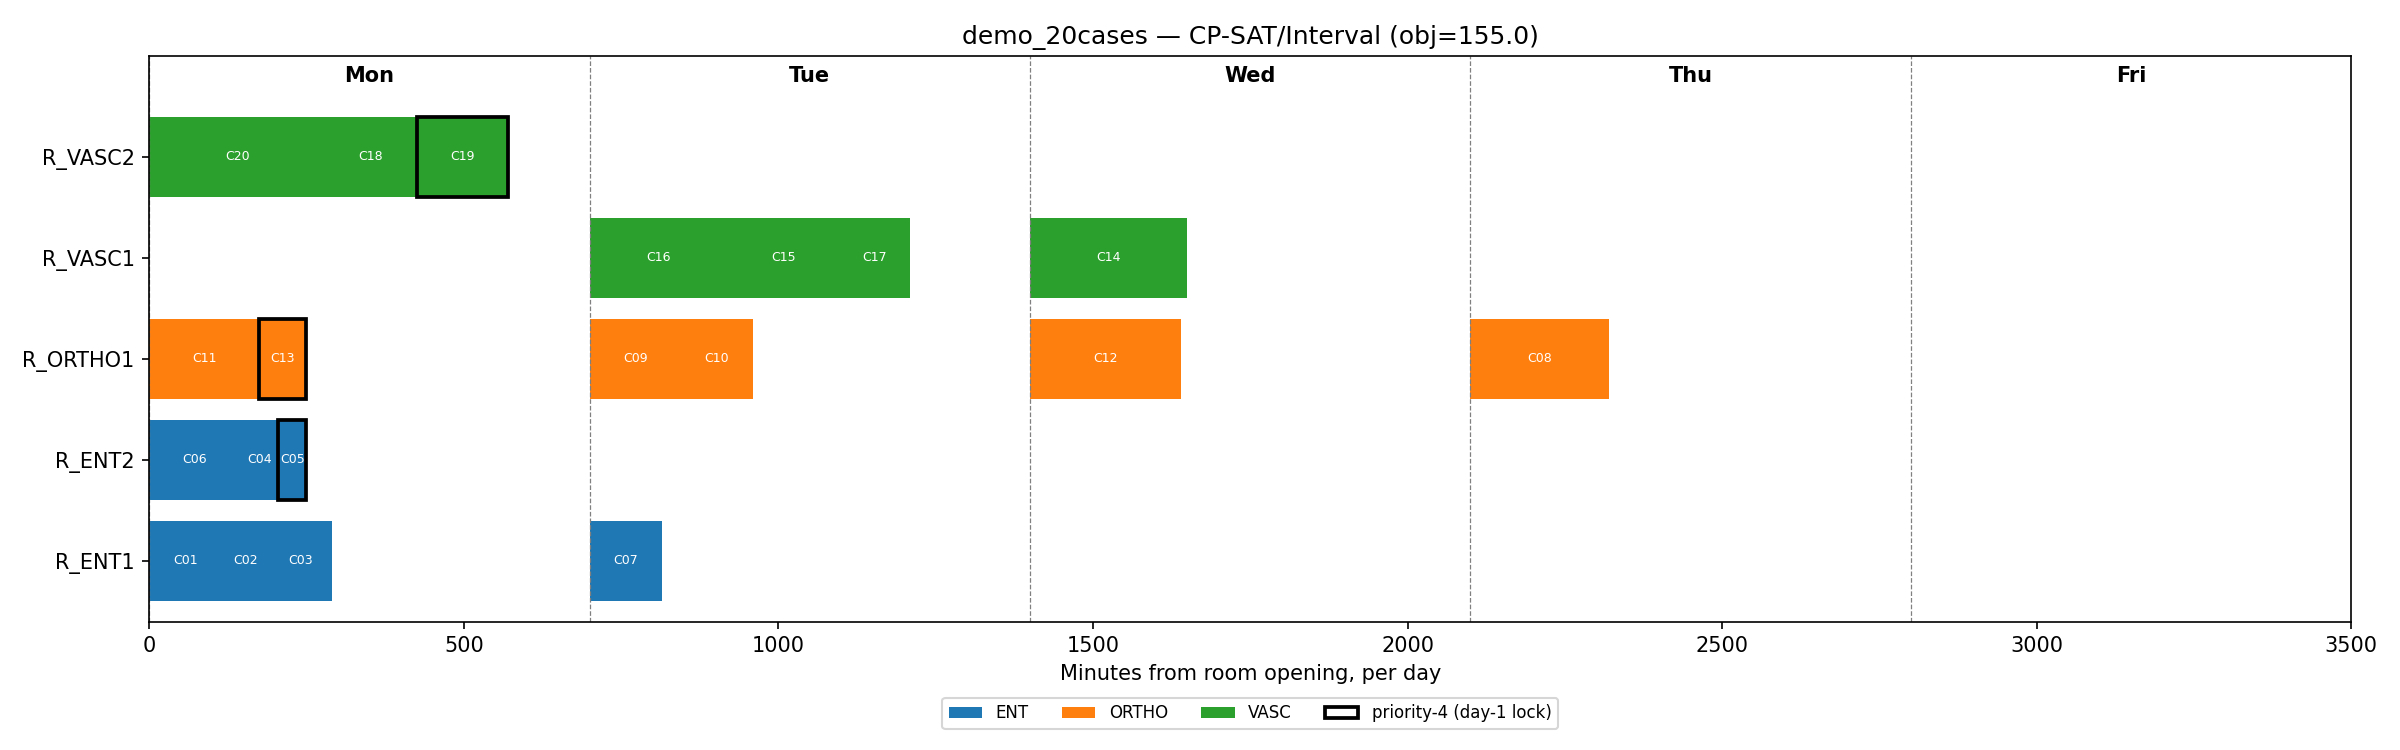
\includegraphics[width=0.96\linewidth]{img/demo_cp_sat.png}
  \end{center}
  \footnotesize \textbf{Leitura:} cada linha é um bloco; cada barra é um
  caso, colorida por serviço. Barras com contorno a negrito são casos
  prioridade-4, bloqueados à 2\textordfeminine\ feira. Notar na
  \textbf{3\textordfeminine\ feira}: R\_VASC1 e R\_VASC2 têm cada um
  um caso do intensificador -- o planificador identificou correctamente que
  nunca se sobrepõem em tempo, mesmo que ambos caiam no mesmo dia.
\end{frame}

\begin{frame}{Demo -- Gantt MIP de comparação}
  \begin{center}
    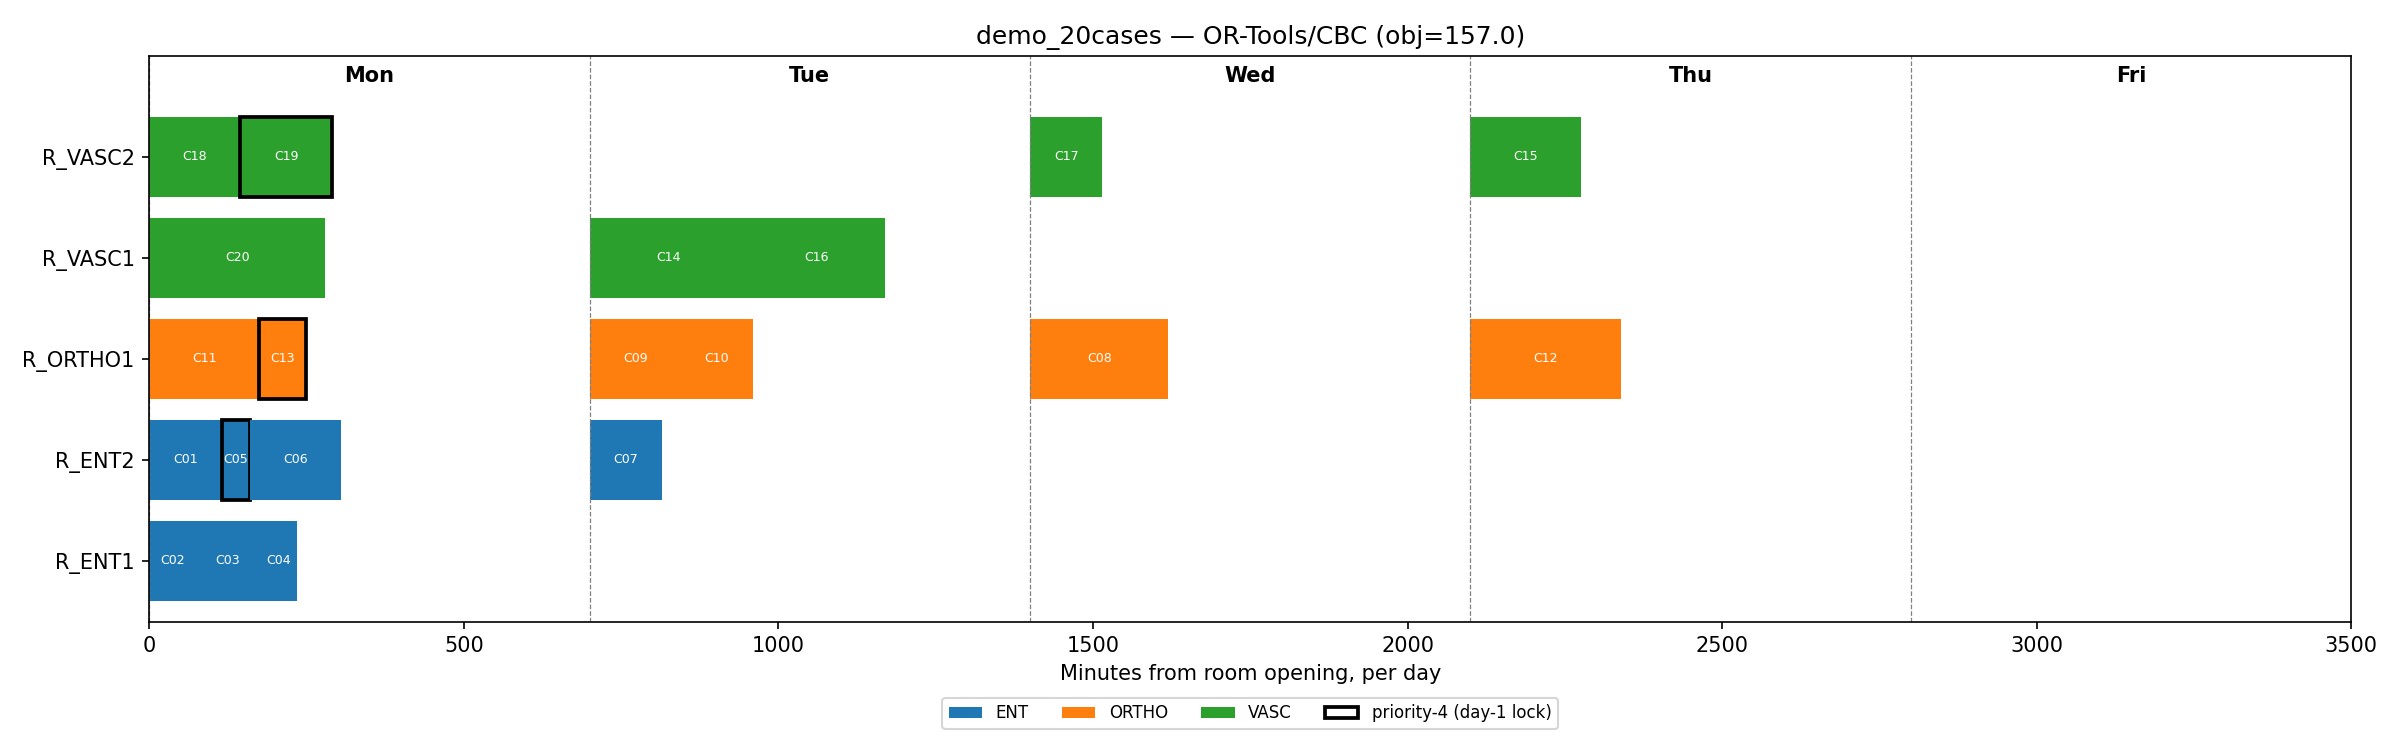
\includegraphics[width=0.96\linewidth]{img/demo_baseline_milp.png}
  \end{center}
  \footnotesize \textbf{Leitura:} os mesmos casos, os mesmos serviços.
  O MIP não tem horas exactas (formulação por dia-balde) -- os casos
  são dispostos consecutivamente apenas para visualização. Comparar a
  distribuição do intensificador: cada dia (2\textordfeminine\ a
  5\textordfeminine\ feira) tem exactamente um caso. A restrição de
  contagem diária está satisfeita, mas produz um agendamento
  desnecessariamente distribuído -- região viável menor, não uma pesquisa pior.
\end{frame}

\begin{frame}{Instância média -- resultados (200 casos, 2 minutos)}
  \footnotesize
  \textbf{Passo 1 -- óptimo real do MIP} via Gurobi (desfasamento próximo
  de zero): \textbf{74\,074.0}, 130/200 agendados, em $<1$ segundo.

  \textbf{Passo 2 -- orçamento realista de 2 minutos / 1\% de desfasamento:}

  \begin{center}
  \begin{tabular}{lccccc}
    \toprule
    Solver & Estado & Objectivo & Desf. próprio & vs. óptimo real & Agend. \\
    \midrule
    Gurobi (referência) & Óptimo & 74\,074.0 & 0.00\% & --- & 130/200 \\
    OR-Tools/CBC & Viável & 74\,116.0 & 0.56\% & $+0.06\%$ & 130/200 \\
    \textbf{CP-SAT} & Viável & \textbf{69\,956.0} & 6.62\% & \textbf{$-5.56\%$} & \textbf{131/200} \\
    \bottomrule
  \end{tabular}
  \end{center}
  \vspace{0.4em}
  O CBC atinge o óptimo provado do MIP em 2 minutos. O CP-SAT
  \textbf{supera esse óptimo em 5.56\%} agendando mais um caso -- está
  a pesquisar uma região viável estritamente maior e correcta, não uma
  pesquisa pior. O desfasamento próprio (6.62\%) é relativo à sua
  própria fronteira -- um espaço maior é mais difícil de fechar.
\end{frame}

\begin{frame}{Instância média -- Gantt CP-SAT (200 casos)}
  \begin{center}
    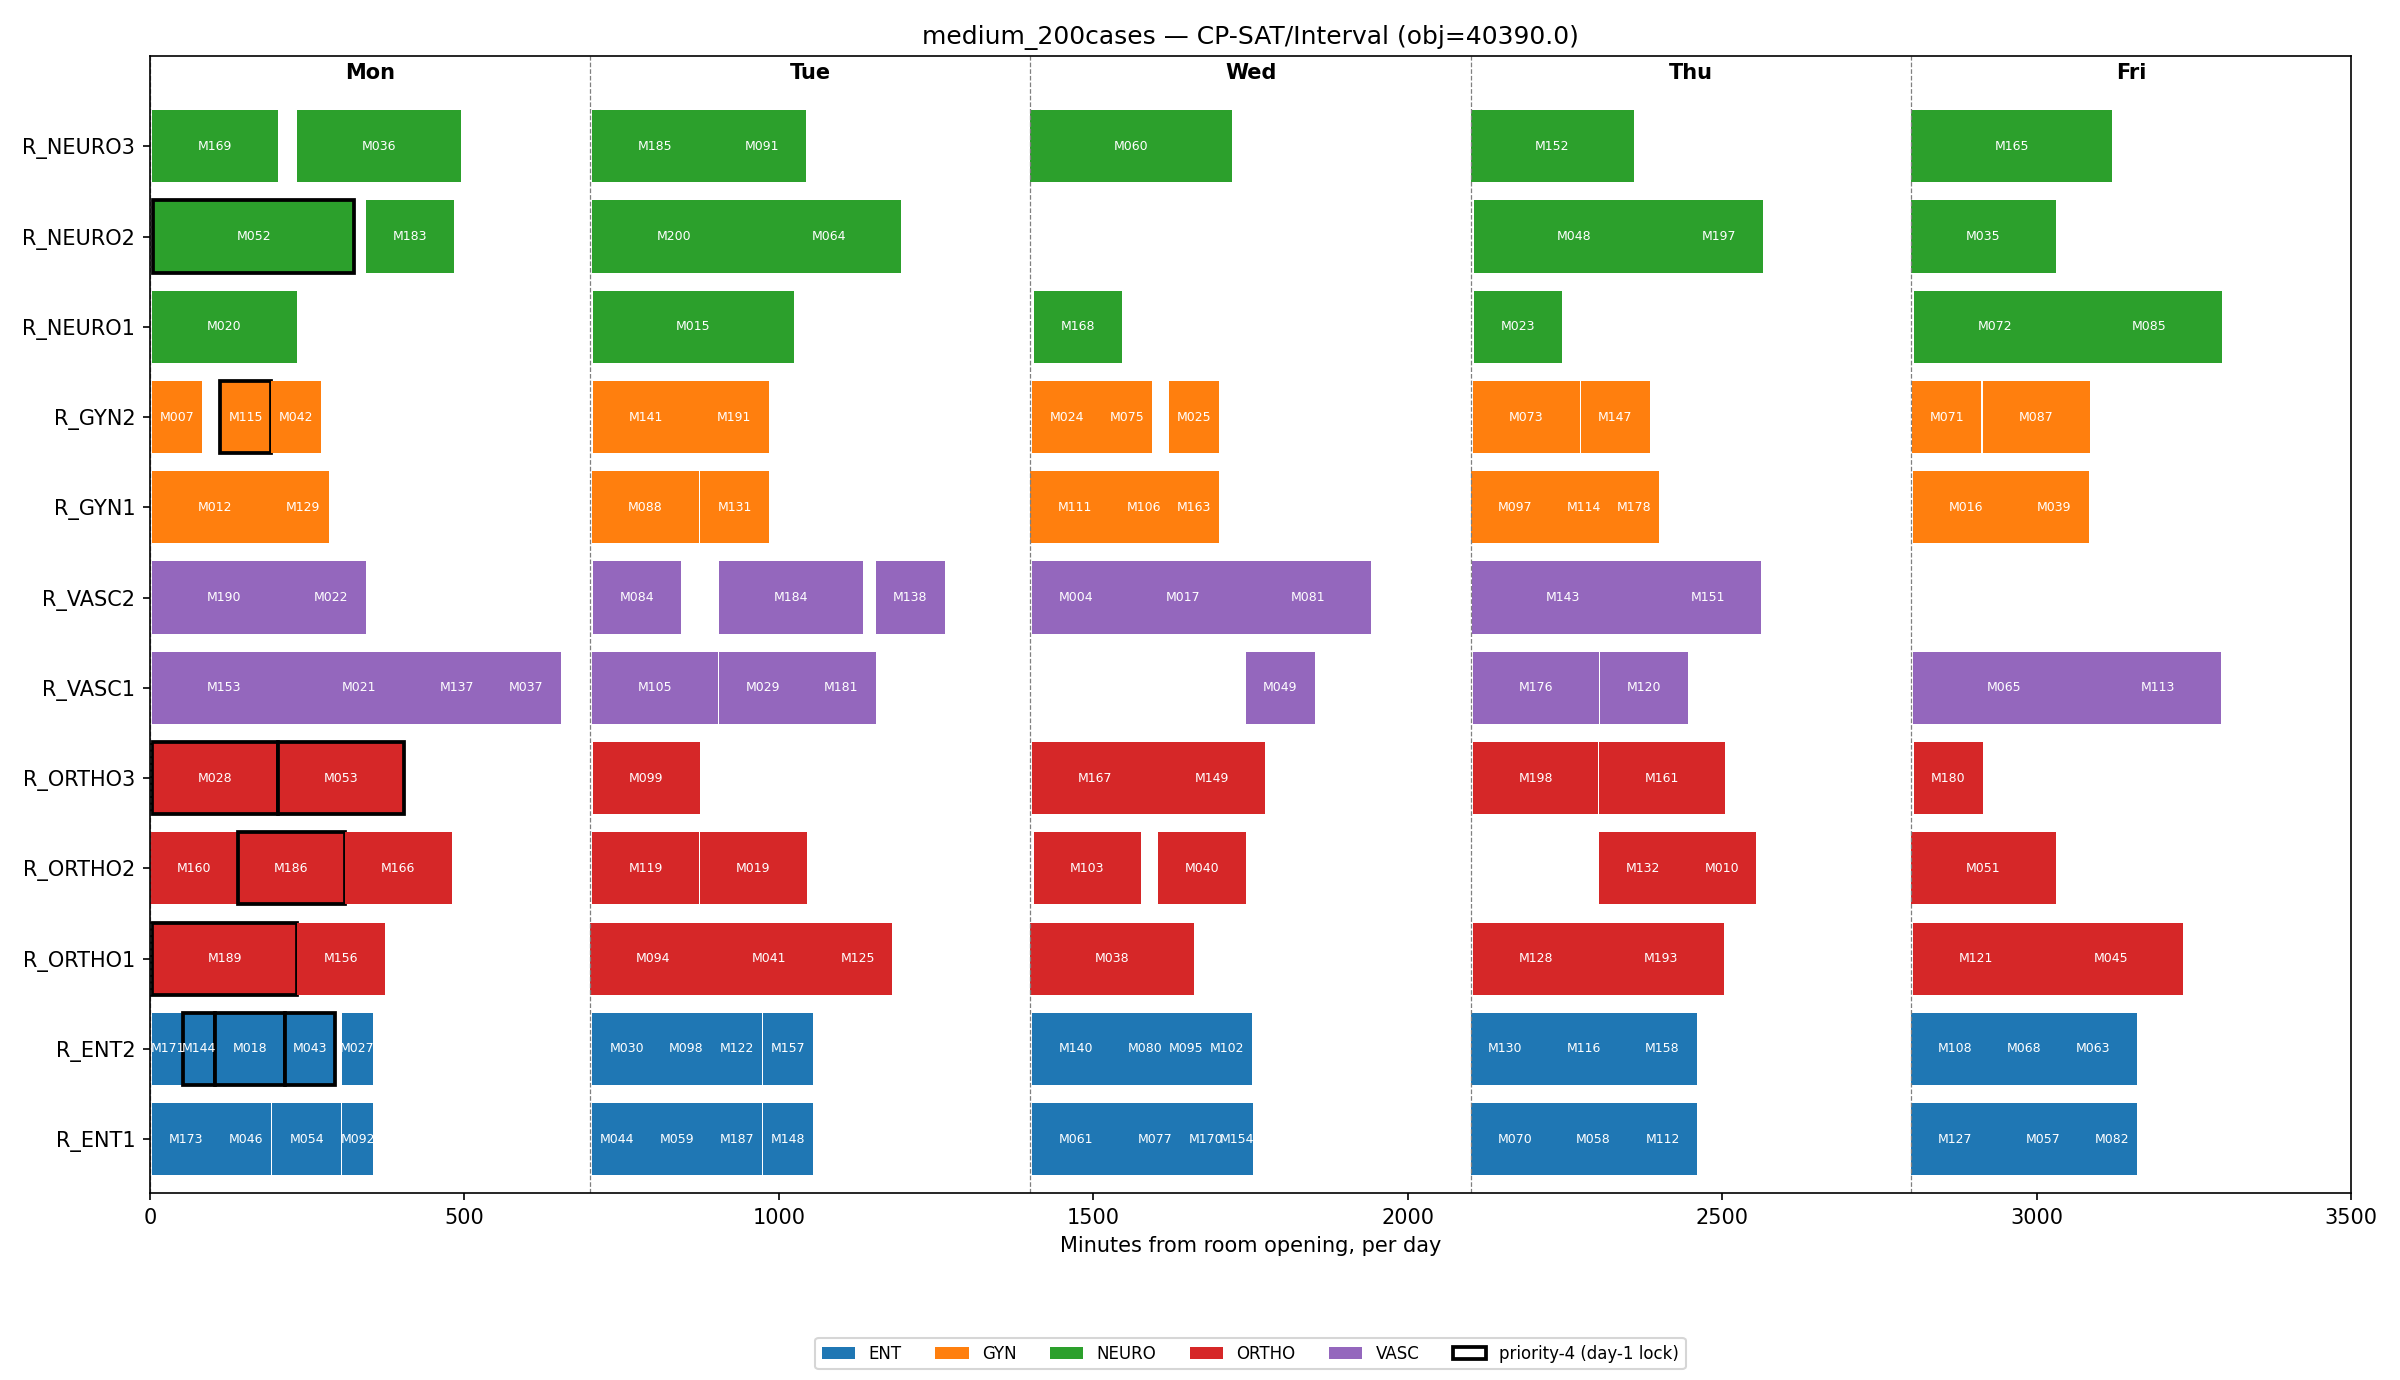
\includegraphics[width=0.96\linewidth]{img/medium_cp_sat.png}
  \end{center}
  \footnotesize \textbf{Leitura:} 12 blocos (linhas), 5 dias,
  $\sim$131 casos agendados com horas de início e fim exactas por caso.
  A densidade e variedade do agendamento mostra o modelo a raciocinar
  simultaneamente sobre os cinco serviços, com restrições de equipamento
  partilhado activas nos blocos VASC e NEURO.
\end{frame}

% ============================================================
\section{Deployment em Produção}

\begin{frame}{O que mudaria num deployment real}
  \small
  \begin{enumerate}
    \item \textbf{Carregador de dados}: mapear a exportação EHR/PAS do
      hospital para \texttt{PlanningInstance}. O esquema alinha com os
      conjuntos de dados CC~BY~4.0 de Akbarzadeh \& Maenhout (2023).
    \item \textbf{Calibração de parâmetros}:
      \begin{itemize}\footnotesize
        \item $\text{wl}^{max}_p$: metas de espera publicadas pelo próprio hospital
        \item $k_{hd}/k_h$: comprimentos de sessão do plano de trabalho dos cirurgiões
        \item $\mu_p$: elicitação estruturada com chefes de serviço (ancorada
          em cenários, não em multiplicadores)
        \item $\beta_\rho$, $\kappa_{ed}$: censo real de camas e inventário de equipamento
      \end{itemize}
    \item \textbf{Cadência semanal}: executar com orçamento de 30 min a 2 horas;
      resultados de 2 minutos já demonstram superação de 5.56\% do óptimo MIP.
    \item \textbf{Testes de aceitação}: estender \texttt{tests/test\_model.py}
      com retrospecção de dados reais; qualquer reimplementação deve passar
      as mesmas verificações de restrições fortes.
    \item \textbf{Monitorização de equidade}: acompanhar a quota de
      incumprimento por serviço em paralelo com o objectivo agregado.
  \end{enumerate}
\end{frame}

% ============================================================
\section{Arquitectura e Reutilização}

\begin{frame}{Como o projecto está construído}
  \small
  \begin{itemize}
    \item \textbf{CP-SAT} (\texttt{cp\_sat\_interval\_solver.py}) -- o
      modelo, backend por defeito, o único necessário para executar.
    \item \textbf{MIP de comparação} (\texttt{milp\_baseline\_solver.py}) --
      CBC / SCIP / Gurobi / CPLEX; mantido apenas como evidência empírica
      para a escolha CP.
    \item \textbf{CP Optimizer} (\texttt{cp\_optimizer\_solver.py}) --
      opcional, licença necessária; adiciona limpeza dependente da sequência;
      retrocede automaticamente para CP-SAT.
    \item \texttt{src/model/types.py} -- dicionário de dados independente
      do solver; cada símbolo matemático mapeia para um campo.
    \item \texttt{src/model/penalty.py} -- uma implementação de $w_c$,
      partilhada por todos os backends.
    \item \texttt{tests/test\_model.py} -- contrato de aceitação: restrições
      fortes verificadas na saída de cada solver em cada execução.
  \end{itemize}
\end{frame}

\begin{frame}{Diagrama do pipeline de integração CP-SAT}
  \centering
  \begin{tikzpicture}[
    node distance=0.28cm and 0.42cm,
    proc/.style={draw, rectangle, rounded corners=2pt,
                 fill=blue!10, align=center, font=\tiny,
                 minimum width=2.55cm, minimum height=0.62cm},
    io/.style={draw, rectangle, rounded corners=2pt,
               fill=green!15, align=center, font=\tiny,
               minimum width=2.55cm, minimum height=0.62cm},
    warn/.style={draw, rectangle, rounded corners=2pt,
                 fill=orange!18, align=center, font=\tiny,
                 minimum width=2.55cm, minimum height=0.62cm},
    outnode/.style={draw, rectangle, rounded corners=2pt,
                fill=teal!18, align=center, font=\tiny,
                minimum width=2.55cm, minimum height=0.62cm},
    arr/.style={-{Stealth[length=3pt,width=2pt]}, thick},
    backloop/.style={-{Stealth[length=3pt,width=2pt]}, thick, dashed, red!60!black},
  ]
    \node[io]   (A) {Dados do hospital\\EHR / PAS};
    \node[proc, right=of A] (B) {Construir\\PlanningInstance};
    \node[proc, right=of B] (C) {Calcular $dd_c$, $w_c$\\prioridade e penalidade};
    \node[proc, right=of C] (D) {Pré-filtro C4--C6\\$(c,d,r)$ elegíveis};
    \node[proc, right=of D] (E) {Criar variáveis\\$\text{pr}$, $\text{start}$, $\text{iv}$,\\$\text{sgiv}$, $u_c$, $\text{bed}_c$};

    \node[proc, below=0.75cm of E] (F) {Adicionar C1--C11\\NoOverlap, Cumulativo,\\limites de soma};
    \node[proc, left=of F] (G) {Definir objectivo\\4 termos};
    \node[warn, left=of G] (H) {Pesquisa CP-SAT\\portfólio paralelo\\desf. $\le1\%$ / tempo};
    \node[proc, left=of H] (I) {Extrair solução\\agendados + não agend.};
    \node[outnode, left=of I] (J) {Verificar C1--C11\\+ output Gantt};

    \draw[arr] (A)--(B); \draw[arr] (B)--(C);
    \draw[arr] (C)--(D); \draw[arr] (D)--(E);
    \draw[arr] (E)--(F);
    \draw[arr] (F)--(G); \draw[arr] (G)--(H);
    \draw[arr] (H)--(I); \draw[arr] (I)--(J);
    \draw[backloop] (H.north) -- ++(0,0.35) -- node[above,font=\tiny,text=black]{continua internamente} ++(-2.6cm,0) -- (G.north);
  \end{tikzpicture}

  \vspace{0.3em}
  \footnotesize Cada caixa corresponde a um ficheiro no repositório.
  O pré-filtro (C4--C6) é executado uma vez na construção -- nunca repetido.
  O portfólio paralelo no passo de pesquisa usa $\le$\texttt{cpu\_count()} trabalhadores;
  partilham cláusulas aprendidas entre si.
\end{frame}

\begin{frame}{Uma biblioteca reutilizável de modelos (Resposta Q\&A 2)}
  \begin{enumerate}\small
    \item \textbf{Tipos de dados base} -- dataclasses tipadas, sem
      importações de solver; todos os modelos na biblioteca assentam nelas.
    \item \textbf{Padrões de restrições} -- somas de capacidade,
      não-sobreposição via NoOverlap, objectivo de tardança por prioridade,
      pré-filtro de elegibilidade. O escalonamento de enfermeiros e a
      alocação de camas precisam das mesmas \emph{formas}, não do mesmo
      modelo.
    \item \textbf{Templates de problemas} -- compõem esses padrões numa
      formulação específica. Este projecto é um template.
    \item \textbf{Camada de adaptação de solver} -- um ficheiro por família
      de backend (MILP, CP, pesquisa local); um novo problema escolhe um
      backend sem reescrever a lógica de restrições.
  \end{enumerate}
  \vspace{0.4em}
  A comparação empírica CP-vs-MIP que este projecto executa é ela própria
  o template para a camada 4: \emph{argumentar} a escolha de backend a
  partir da estrutura do problema, \emph{verificar} numa instância pequena,
  depois comprometer.
\end{frame}

\begin{frame}{Passar o testemunho (Resposta Q\&A 1)}
  \begin{enumerate}\small
    \item \textbf{FORMULATION.md + FORMULATION\_CP.md}: enquadramento,
      evidência, pressupostos, todos os conjuntos/parâmetros/variáveis/
      restrições com matemática completa. Uma fonte de verdade.
    \item \textbf{\texttt{src/model/types.py}}: as dataclasses \emph{são}
      o dicionário de dados -- cada símbolo matemático mapeia exactamente
      para um campo.
    \item \textbf{Código do solver com números C}: cada restrição em
      \texttt{cp\_sat\_interval\_solver.py} tem a etiqueta C1\ldots C11,
      coincidindo com FORMULATION\_CP.md -- lidos em paralelo, sem
      ambiguidade.
    \item \textbf{\texttt{tests/test\_model.py}}: barra de aceitação --
      qualquer reimplementação deve passar as mesmas verificações de
      restrições fortes na instância demo; escrever um novo teste com
      cada nova restrição.
    \item \textbf{Um glossário curto}: a maior parte da confusão neste
      tipo de projecto é vocabulário (``escala de bloco'', ``ambulatório'',
      o que significa P4 operacionalmente), não matemática.
  \end{enumerate}
\end{frame}

\begin{frame}{Para onde levaria isto a seguir}
  \small
  \begin{center}
  \begin{tabular}{ll}
    \toprule
    Extensão & Abordagem \\
    \midrule
    Durações estocásticas & PL estocástica de 2 estágios \\
    Reagendamento intra-dia & LNS com semente no plano actual \\
    Reserva de capacidade para urgências & Bloco de capacidade por dia fora do modelo electivo \\
    Escalonamento de enf./anest. & Estender $H$, reutilizar padrão NoOverlap/cap dos cirurgiões \\
    Horizonte multi-semana & Transportar não agendados com prioridade aumentada \\
    Capacidade de camas variável por dia & \texttt{Cumulative} segmentado por dia \\
    Equidade por especialidade & Objectivo secundário limitando quota de incumprimento \\
    Piloto com dados reais & Conjuntos de dados CC~BY~4.0 Akbarzadeh \& Maenhout \\
    \bottomrule
  \end{tabular}
  \end{center}
\end{frame}

\begin{frame}{Conclusões: o que as experiências demonstram}
  \small
  \begin{enumerate}
    \item \textbf{O CP-SAT encontra agendamentos estritamente melhores em
      ambas as instâncias.} Demo: 155.0 vs. 157.0 (MIP). Instância média:
      69\,956 vs. 74\,074 (óptimo \emph{provado} do MIP) -- melhoria de
      5.56\% agendando mais um caso. A razão é sempre a mesma: região
      viável maior e correcta.
    \item \textbf{O desfasamento próprio não mede o que parece.} O
      desfasamento de 6.62\% do CP-SAT e o de 0.56\% do CBC são medidos
      face a fronteiras de \emph{regiões viáveis diferentes}. A comparação
      correcta é o valor absoluto do objectivo; o CP-SAT ganha claramente.
    \item \textbf{A modelação do equipamento partilhado é o factor estrutural
      decisivo.} \texttt{AddCumulative} verifica sobreposição temporal real;
      a contagem diária do MIP proíbe dois casos sequenciais do intensificador
      C no mesmo dia mesmo quando nunca se sobrepõem.
    \item \textbf{C11 (camas de recuperação/UCI) não pode ser expressa num MIP
      de dia-balde.} Só este facto é justificação estrutural para CP baseado
      em intervalos, independentemente do desempenho.
    \item \textbf{O design de dois intervalos permite práticas reais de bloco
      operatório.} O cirurgião livre em $t=70$ pode entrar num segundo bloco
      enquanto o Bloco 1 ainda está a ser limpo até $t=90$.
    \item \textbf{A instância demo resolve em $\sim$0.1 s com zero desfasamento
      provado} -- inteiramente prático mesmo para suporte a decisão em tempo real.
    \item \textbf{Com um orçamento de 2 minutos, o CP-SAT já é mais valioso
      que o CBC.} Mais casos agendados, objectivo menor, mesmo tempo de execução.
  \end{enumerate}
\end{frame}

\begin{frame}{Questões}
  \centering
  \Large Obrigado.
  \vspace{1em}
  \normalsize
  \hyperlink{toc}{\beamergotobutton{Voltar à agenda}}
  \quad
  \hyperlink{mip1}{\beamergotobutton{Apêndice MIP completo}}
\end{frame}

% ============================================================
\appendix
\section{Apêndice: Modelo MIP de Comparação}

\begin{frame}{MIP -- visão geral da formulação}
  \hypertarget{mip1}{}
  O MIP de comparação (FORMULATION.md, Apêndice A) é implementado em
  \texttt{milp\_baseline\_solver.py} e executa via
  \texttt{-{}-solver milp-cbc} (incluído), \texttt{milp-gurobi}, ou
  \texttt{milp-cplex} (licença comercial necessária).

  \textbf{Igual ao CP-SAT}: conjuntos, pré-filtro de elegibilidade (C4--C6),
  prioridades, $w_c$ do mesmo \texttt{penalty.py}.

  \textbf{Diferenças principais}:
  \begin{itemize}\small
    \item Sem horas exactas intra-dia -- decisões ao nível de \emph{dia+bloco}.
    \item C7 e C10 são somas de capacidade lineares, não sobreposição exacta.
    \item C11 (camas de recuperação) \emph{não é expressável} -- uma variável
      de dia-balde não tem valor de ``dia de cirurgia''.
    \item Sem Termo 4 no objectivo.
  \end{itemize}
  \bk
\end{frame}

\begin{frame}{MIP -- variáveis, referência completa}
  \footnotesize
  \begin{center}
  \begin{tabular}{p{2.4cm}p{2.8cm}p{6.5cm}}
    \toprule
    \textbf{Variável} & \textbf{Domínio} & \textbf{Significado} \\
    \midrule
    $x_{cdr}$ & $\{0,1\}$ &
      1 se o caso $c$ é agendado no dia $d$ no bloco $r$.
      Apenas criada para trios elegíveis (mesmo pré-filtro C4--C6 do CP-SAT).
      Determina o dia e o bloco, mas \emph{não} a hora exacta. \\[3pt]
    $z_c$ & $[0,1]$ &
      1 se o caso $c$ \emph{não} é agendado esta semana (só para
      $p_c\ne4$). Declarada contínua -- C3 força-a a $\{0,1\}$ no óptimo
      porque o objectivo penaliza não-agendamento fraccionário; declará-la
      binária não acrescenta nenhum apertamento à relaxação LP. \\
    \bottomrule
  \end{tabular}
  \end{center}
  \vspace{0.4em}
  \textbf{Objectivo} (mesma estrutura de três termos que o CP-SAT, sem Termo 4):
  \[\footnotesize
    \min\;\sum_{c:\,dd_c\ge0}\sum_{d,r}[dd_c+d]\,x_{cdr}
    +\sum_{c:\,dd_c<0}\sum_{d,r}[dd_c+\alpha d]\,x_{cdr}
    +\sum_{c:\,p_c\ne4}w_c\,z_c
  \]
  O mesmo \texttt{penalty.py} calcula $w_c$ -- sem implementação separada
  por solver. Sem Termo 4 porque C11 não é expressável.
  \bk
\end{frame}

\begin{frame}{MIP -- restrições e o que está em falta}
  \textbf{C7 (bloco, soma agregada):}
  \[\small
    \sum_{c\in C}t_c^{tot}\,x_{cdr}\le k_{dr}\qquad\forall d,r
  \]
  Para um único bloco: equivalente à não-sobreposição exacta. Para um
  \emph{recurso partilhado entre blocos}: conta incorrectamente todos
  os usos do equipamento como se se sobrepusessem.

  \textbf{C10 (equipamento, contagem diária):}
  \[\small
    \sum_{c:\,u_{ce}=1}\sum_r x_{cdr}\le\kappa_{ed}\qquad\forall e,d
  \]
  Conta \emph{quantos} casos do equipamento $e$ caem num dia, não se
  se sobrepõem -- principal fonte do desfasamento de 5.56\% no objectivo.

  \textbf{Sem C11:} ``$\text{bed}_c$ começa no dia em que $c$ é agendado''
  não pode ser escrito -- nenhuma variável num modelo de dia-balde guarda
  o ``dia de cirurgia'' como \emph{valor}.
  \bk
\end{frame}

\begin{frame}{CP Optimizer (opcional, apêndice)}
  \small Mantido por uma razão: \textbf{limpeza dependente da sequência}
  -- uma matriz de transição entre casos adjacentes num bloco via
  \texttt{sequence\_var + no\_overlap(transition\_matrix)}.
  \begin{center}
  \begin{tabular}{lcc}
    \toprule
    & Mesmo serviço & Serviço diferente \\
    \midrule
    CP-SAT (por escalão de duração) & $t_c^{clean}$ do próprio caso & igual \\
    CP Optimizer & 15 min & 35 min \\
    \bottomrule
  \end{tabular}
  \end{center}
  Instância demo: idêntico ao CP-SAT (155.0, 20/20, Óptimo) -- confirmado
  que os intervalos de limpeza do mesmo serviço são exactamente 15 min.
  \bk
\end{frame}

\begin{frame}{Referências}
  \tiny
  \begin{enumerate}
    \item Cardoen, B., Demeulemeester, E., \& Beli\"en, J. (2010).
      Operating room planning and scheduling: A literature review.
      \emph{EJOR}, 201(3), 921--932.
      \texttt{doi:10.1016/j.ejor.2009.04.011}
    \item Marques, I., \& Captivo, M.E. (2015).
      \emph{Planeamento de cirurgias el\'etivas no Centro Hospitalar
      Lisboa Norte}. Dissertação de mestrado, Universidade de Lisboa.
    \item Denton, B.T., Miller, A.J., Balasubramanian, H.J., \&
      Huschka, T.R. (2010). Optimal allocation of surgery blocks to
      operating rooms under uncertainty. \emph{Oper.\ Res.}, 58(4),
      802--816. \texttt{doi:10.1287/opre.1090.0791}
    \item SIGIC -- Portaria n.\textsuperscript{o} 45/2008, Di\'ario da
      Rep\'ublica, Portugal.
    \item Van Riet, C., \& Demeulemeester, E. (2015). Trade-offs in
      operating room planning for electives and emergencies.
      \emph{OR Spectrum}, 37(1), 59--87.
      \texttt{doi:10.1007/s00291-013-0345-2}
    \item Macario, A. (2010). What does one minute of operating room
      time cost? \emph{J.\ Clin.\ Anesth.}, 22(4), 233--236.
      \texttt{doi:10.1016/j.jclinane.2010.02.003}
    \item Akbarzadeh, B., \& Maenhout, B. (2023a). Real life data for
      OR scheduling problem. Mendeley Data V2.
      \texttt{doi:10.17632/n2v49z2vnp.2}
    \item Akbarzadeh, B., \& Maenhout, B. (2023b). RealLife OR
      scheduling dataset, 2021-Jan-May. Mendeley Data V1.
      \texttt{doi:10.17632/c8d342266x.1}
    \item Perron, L., \& Furnon, V. \emph{CP-SAT: a CP Solver}.
      Google OR-Tools.
      \texttt{developers.google.com/optimization/cp}
    \item Baptiste, P., Le Pape, C., \& Nuijten, W. (2001).
      \emph{Constraint-Based Scheduling}. Kluwer.
      \texttt{doi:10.1007/978-1-4615-1479-4}
    \item Vil\'im, P. (2004). $O(n\log n)$ filtering for unary
      resource constraints. \emph{CPAIOR 2004}.
      \texttt{doi:10.1007/978-3-540-24664-0\_15}
    \item Schutt, A., Feydy, T., Stuckey, P.J., \& Wallace, M.G.
      (2009). Why cumulative decomposition is not as bad as it sounds.
      \emph{CP 2009}. \texttt{doi:10.1007/978-3-642-04244-7\_45}
    \item Laborie, P. (2009). IBM ILOG CP Optimizer for detailed
      scheduling illustrated on three problems. \emph{CPAIOR 2009}.
      \texttt{doi:10.1007/978-3-642-01929-6\_5}
  \end{enumerate}
  \bk
\end{frame}

\end{document}
